\documentclass[10pt,a4paper]{article}
\usepackage[margin=25mm]{geometry}
\usepackage[T1]{fontenc}
\usepackage{mathptmx}
\renewcommand{\ttdefault}{lmtt}
\usepackage{url}
\usepackage{graphicx,booktabs,amsmath,microtype,caption,url}
\captionsetup{font=small,labelfont=bf}
\setlength{\parskip}{0pt}
\title{\bfseries Evolutionary Linear Merging of Eight Qwen3.5-4B Fine-Tunes\\with a Generation-Based, Token-Capped Fitness:\\Baphomet-1.1-4B\\[2pt]\large Technical Report (revised with rounds 2--3)}
\author{CloudGoat}
\date{November 2026}
\begin{document}
\maketitle

\begin{abstract}
We search the linear merge coefficients of eight fine-tunes of Qwen3.5-4B with an EvoGM-style evolutionary procedure, using as fitness the plain accuracy of \emph{generated} answers (chat template, thinking enabled, 4{,}096-token cap) on 110 held-out items from MMLU-Pro, GPQA and BFCL. A first round (40 candidates, 7.1 T4-GPU hours) produced a merge that matched the hand-set uniform merge Baphomet-1.0-4B ($\lambda_i=0.1375$) on a disjoint 180-item test (77.2\% vs.\ 77.8\%) at half the completion tokens. We then continued the search for two more rounds with an IRT-accelerated fitness: a 40-item subset scored with per-task 2PL models, early stopping of weak candidates, and exact 110-item re-evaluation of the most promising ones (6.53 GPU hours). The round-3 winner, released as \textbf{Baphomet-1.1-4B}, reaches a fitness of 0.764 (round-1 winner 0.722, best single donor 0.686, Baphomet-1.0 0.603) and is the numerically best model on the 180-item test: 79.4\% vs.\ 77.8\% for Baphomet-1.0 and 70.0\% for the base model. The gain over Baphomet-1.0 is not significant (10 vs.\ 7 discordant items, McNemar $p=0.63$); the gain over the base model is (20 vs.\ 3, $p<0.001$). Baphomet-1.1 uses 42\% fewer completion tokens than Baphomet-1.0 (1{,}834 vs.\ 3{,}180) but more than the round-1 winner (1{,}498). The fitness is a single sample at temperature 0.6, the winner was selected on it, and the test set is small, so these results are preliminary.
\end{abstract}

\section{Introduction}
Task-arithmetic merging adds weighted task vectors $\tau_i=\theta_i-\theta_0$ of fine-tuned models to a shared base $\theta_0$. The weights $\lambda_i$ are usually set by hand. Baphomet-1.0-4B is such a merge: eight Qwen3.5-4B fine-tunes combined with equal weights. Evolutionary search can tune $\lambda$ automatically, but its outcome depends heavily on the fitness signal. In an earlier attempt (MERGE$^3$-style search with log-likelihood multiple-choice fitness, no chat template, MMLU-Pro and GPQA only), the evolved merge lost clearly to Baphomet on generated answers and degraded tool calling.

This report revisits the problem with a fitness that measures what the model is actually used for: generated answers with the chat template and thinking enabled, including a tool-calling task, under a fixed token budget. We ask (i) whether evolved coefficients beat the uniform merge, and (ii) what kind of merge the search prefers. Sections~\ref{sec:r1setup}--\ref{sec:r1res} describe the first search round; Sections~\ref{sec:r2}--\ref{sec:r2res} describe two further rounds with an IRT-accelerated fitness, whose winner is released as Baphomet-1.1-4B.

\section{Setup}\label{sec:r1setup}
\paragraph{Models.} Base: Qwen/Qwen3.5-4B~\cite{qwen}. Reference: Baphomet-1.0-4B~\cite{baph}, the uniform merge. The final model of this report, Baphomet-1.1-4B, is the EvoGM round-3 winner (Section~\ref{sec:r2res}). Donors (in coefficient order): Agents-A1, DeepSeek-V4-Pro distill (\textit{dsv4pro}), Qwen3.8-Distill (\textit{q38distill}), Qwopus-Coder, Qwopus-v3, AREX-Turbo, NeoHorse and T-Max~\cite{m1,m2,m3,m4,m5,m6,m7,m8}, all 4B fine-tunes of the same base. Parameters missing from a donor (e.g.\ MTP heads, vision tower) contribute zero.

\paragraph{Merge.} $\theta=\theta_0+\sum_{i=1}^{8}\lambda_i\tau_i$, $\lambda_i\in[-1,1]$, fp32 accumulation. Task vectors are stored in fp8 during the search; our reconstruction of Baphomet agrees with the published weights to within one bf16 ulp. Merged weights are streamed into a persistent vLLM engine in place.

\paragraph{Search.} A port of the EvoGM~\cite{evogm} reference implementation~\cite{evogmcode} (dual MLP generators mapping losers to winners with cycle consistency; Adam, lr $10^{-4}$, 200 epochs per iteration; winners = top 30\%). The initial population contains the eight one-hot vectors, the uniform average ($1/8$), and Baphomet's coefficients. EvoGM uses two nested loops. Each iteration (inner loop) trains the generators, proposes new candidates and keeps the top $P$; each round (outer loop) groups the iterations and ends with a basis shift, replacing the experts with the top-8 candidates. We ran population size $P=10$, one round (outer loop) of three iterations (inner loop), seed 42: 40 evaluated candidates in total. With a single round, no basis shift took place (the reference default is two rounds). The run was scaled to fit a 10-GPU-hour budget on 2$\times$T4.

\paragraph{Fitness.} Mean of three accuracies on 110 items: MMLU-Pro (40), GPQA main/extended (30; no Diamond items) and BFCL non-live (40; 10 per category). Generation uses the chat template with thinking, temperature 0.6, top-$p$ 0.95, top-$k$ 20, seed 0, and a 4{,}096-token cap; truncated answers count as wrong. IRT parameters were used only to select informative items, not for scoring.

\paragraph{Test.} 180 items disjoint from the fitness set: MMLU-Pro 80, GPQA 50, BFCL 50, same decoding but an 8{,}192-token cap. The winner (highest fitness) is compared with Baphomet and the base model on identical items; significance by the exact two-sided McNemar (sign) test on discordant pairs.

\section{Round-1 results}\label{sec:r1res}
\paragraph{Search.} Figure~\ref{fig:traj} shows the trajectory. The best initial member was the single donor q38distill (0.686); Baphomet scored 0.603 and the uniform average 0.592 (Table~\ref{tab:init}). The best fitness rose to 0.697 after iteration 1 and 0.722 after iteration 2; iteration 3 brought no improvement. No candidate failed.

\begin{figure}[htbp]
\centering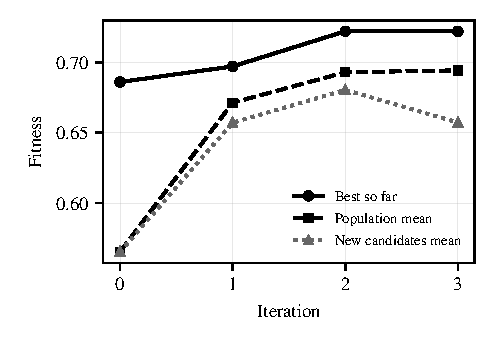
\includegraphics[width=0.55\textwidth]{fig_traj_en.pdf}
\caption{Round 1: fitness per iteration (110 items, 4{,}096-token cap).}
\label{fig:traj}
\end{figure}

\begin{table}[htbp]
\centering\small
\caption{Initial population on the fitness items. Tok.\ = mean completion tokens.}
\label{tab:init}
\begin{tabular}{lcccrr}
\toprule
Candidate & MMLU & GPQA & BFCL & Fit. & Tok. \\
\midrule
q38distill & .70 & .43 & .93 & .686 & 671 \\
dsv4pro & .68 & .47 & .85 & .664 & 1{,}331 \\
Qwopus-v3 & .70 & .23 & .93 & .619 & 1{,}835 \\
Baphomet & .65 & .23 & .93 & .603 & 1{,}925 \\
Average ($1/8$) & .68 & .20 & .90 & .592 & 2{,}073 \\
Qwopus-Coder & .65 & .17 & .88 & .564 & 1{,}834 \\
NeoHorse & .60 & .03 & .90 & .511 & 2{,}180 \\
T-Max & .50 & .13 & .90 & .511 & 2{,}343 \\
AREX-Turbo & .42 & .07 & .95 & .481 & 1{,}924 \\
Agents-A1 & .45 & .07 & .75 & .422 & 2{,}492 \\
\midrule
\textbf{Round-1 winner} & .80 & .47 & .90 & \textbf{.722} & 1{,}096 \\
\bottomrule
\end{tabular}
\end{table}

\paragraph{Winning coefficients.} The round-1 winner is \begin{align*}\lambda^\star = (&0.007,\ 0.104,\ 0.627,\ 0.015,\ 0.233,\ 0.053,\ -0.004,\ 0.010),\end{align*} with most of the weight on q38distill (0.63) and Qwopus-v3 (0.23), a little on dsv4pro (0.10), and near zero elsewhere ($\sum\lambda_i=1.05$, versus 1.10 for Baphomet). The other top candidates also mix mainly dsv4pro, q38distill and Qwopus-v3, the three strongest single donors.

\paragraph{Test set.} Table~\ref{tab:test} (Section~\ref{sec:r2res}) gives the 180-item results. Overall accuracy of the round-1 winner and Baphomet-1.0 is statistically indistinguishable (8 items won, 9 lost, $p=1.0$); per suite, the round-1 winner is ahead on GPQA (+4.0 points) and behind on MMLU-Pro ($-2.5$) and BFCL ($-2.0$), none significant. Against the base model it wins 18 and loses 5 items ($p=0.011$), driven by GPQA (12 vs.\ 2, $p=0.013$).

\paragraph{Reasoning length.} The round-1 winner uses 53\% fewer completion tokens than Baphomet overall, 64\% fewer on MMLU-Pro and 45\% fewer on GPQA, and halves the truncation rate. Across all 40 candidates, fitness and mean completion length are strongly anti-correlated (Spearman $\rho=-0.65$, $p<10^{-5}$; Figure~\ref{fig:scatter}).

\begin{figure}[htbp]
\centering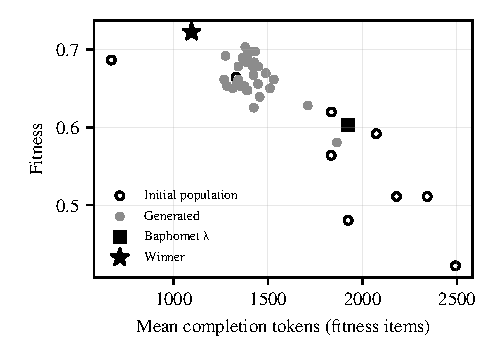
\includegraphics[width=0.55\textwidth]{fig_scatter_en.pdf}
\caption{Round 1: fitness vs.\ mean completion tokens for all 40 candidates.}
\label{fig:scatter}
\end{figure}

\section{Rounds 2--3: IRT-accelerated search}\label{sec:r2}
The first round used the full 110-item fitness for every candidate (about 1{,}000\,s of generation each), which left no budget for EvoGM's outer loop. To continue the search under a further 8-GPU-hour cap, we resumed the saved search state and replaced most full evaluations with a cheaper estimate.

\paragraph{IRT subset and estimator.} The 40 round-1 candidates $\times$ 110 items form a correctness matrix (truncated $=$ wrong). We fit a 2PL item-response model per task (MMLU-Pro, GPQA, BFCL) by joint MAP ($\theta\sim\mathcal N(0,1)$, $\log a\sim\mathcal N(0,0.5^2)$, $b\sim\mathcal N(0,2^2)$) and kept, per task, the items with the highest Fisher information at the abilities of the top-15 candidates divided by $\sqrt{\text{mean tokens}}$: 16 MMLU-Pro + 10 GPQA + 14 BFCL $=$ 40 items (about 66k generated tokens per candidate instead of about 165k). A new candidate answers only these 40 items. Per task, its fitness estimate is the observed number correct on the subset plus the sum of the 2PL probabilities $p(\theta_{\text{MAP}})$ over the unobserved items, divided by the task size; the three task values are averaged, so the estimate is on the same scale as the round-1 fitness. In leave-one-out validation over the 40 round-1 candidates the estimate had a mean absolute error (MAE) of 0.013 against the full fitness (0.009 on the top 15) and a rank correlation of 0.93; the naive subset accuracy had an MAE of 0.066.

\paragraph{Racing.} Outputs are streamed while a candidate is generating. Once at least half of the subset has finished, the controller computes an optimistic estimate ($\theta+1.5\,\text{sd}$) and stops the candidate if it falls below the current $P$-th best population value. In an offline simulation on round-1 iterations 2--3 this pruned 4 of 20 candidates, saved about 9\% of the time and pruned none wrongly.

\paragraph{Completion rule.} To guard against estimation error and the winner's curse, after every iteration the two best not-yet-completed population members are evaluated on the 70 missing items (one per GPU) whenever the best one's estimate is within 0.02 of the best exact fitness so far. This gives their exact 110-item fitness under the round-1 definition. The population and the generators use the best available value (exact if known, otherwise the estimate). The final winner is the candidate with the highest \emph{exact} 110-item fitness over round 1 and all completions; only that candidate is run on the 180-item test.

\paragraph{Search schedule.} Each new round starts with a basis shift: the top-8 candidates of the previous round's history become the new experts (round 2: fitness .722, .703, .697, .697, .692, .692, .689, .686), and the search runs in their coordinates with $P=10$, a fresh generator per round and up to three iterations per round. Rounds and iterations were sized inside the kernel from the measured costs, always reserving time for the final test.

\section{Rounds 2--3: results}\label{sec:r2res}
\paragraph{Run.} The run finished in 6.53 GPU hours on 2$\times$T4 (cap 8\,h). It completed rounds 2 and 3 with three iterations each; round 4 was skipped because the remaining 0.88\,h was less than the 0.92\,h a round needs at minimum. It made 64 new subset evaluations (104 candidates in total with round 1) and 12 completions; 3 candidates were stopped early by racing and none failed.

\paragraph{Search trajectory.} The best exact fitness stayed at the round-1 value 0.722 through round 2 (one completed candidate tied it), rose to 0.733 in round 3, iteration 2, and to 0.764 in round 3, iteration 3 (Figure~\ref{fig:search}, left). Across the 12 completed candidates the IRT estimate had an MAE of 0.009 against the exact fitness, a Spearman correlation of 0.96, and a mean bias of $+0.008$ (Figure~\ref{fig:search}, right). The bias is expected: completions are chosen because their estimates are high. The winner shows it most clearly, with an estimate of 0.782 and an exact fitness of 0.764.

\begin{figure}[htbp]
\centering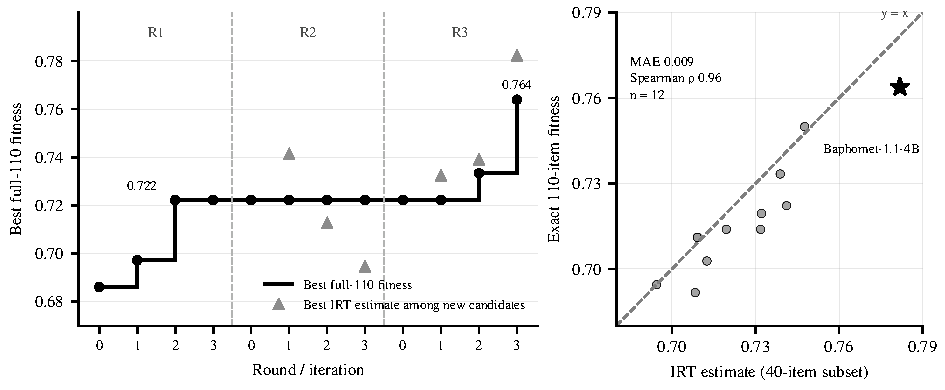
\includegraphics[width=\textwidth]{fig_search_r2_en.pdf}
\caption{Left: best exact 110-item fitness so far after each iteration of rounds 1--3 (iteration 0 $=$ initial population of the round); triangles: best IRT estimate among the new candidates of that iteration (rounds 2--3). Right: IRT estimate vs.\ exact 110-item fitness for the 12 completed candidates; the star is Baphomet-1.1-4B.}
\label{fig:search}
\end{figure}

\paragraph{Baphomet-1.1-4B coefficients.} The round-3 winner is
\begin{align*}\lambda_{1.1} = (&0.0116,\ 0.2039,\ 0.5901,\ 0.0013,\ 0.2972,\ 0.0323,\ 0.0030,\ -0.0007)\end{align*}
over (Agents-A1, dsv4pro, q38distill, Qwopus-Coder, Qwopus-v3, AREX-Turbo, NeoHorse, T-Max), $\sum\lambda_i=1.14$. Compared with the round-1 winner it keeps the same three donors but moves weight from q38distill (0.63\,$\to$\,0.59) to dsv4pro (0.10\,$\to$\,0.20) and Qwopus-v3 (0.23\,$\to$\,0.30); the other five donors stay near zero (Figure~\ref{fig:lambda}).

\begin{figure}[htbp]
\centering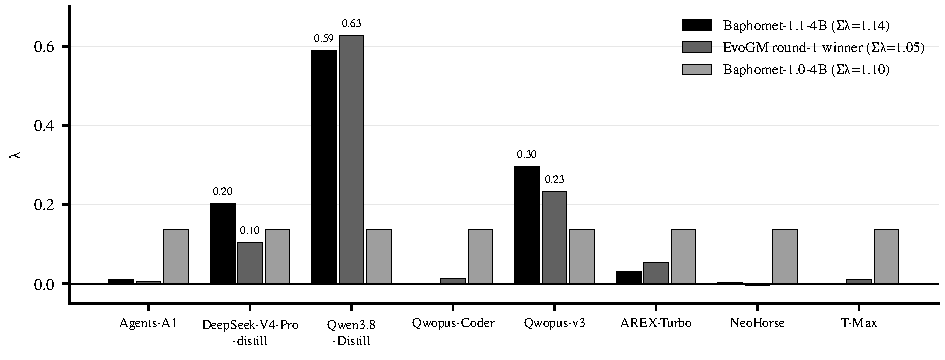
\includegraphics[width=\textwidth]{fig_lambda_en.pdf}
\caption{Merge coefficients of Baphomet-1.1-4B, the round-1 winner and Baphomet-1.0-4B.}
\label{fig:lambda}
\end{figure}

\paragraph{Comparison with the experts on the fitness set.} Table~\ref{tab:fit110} and Figures~\ref{fig:fit110}--\ref{fig:fit110eff} compare Baphomet-1.1 with the eight donors, the uniform average, Baphomet-1.0 and the round-1 winner on the 110 fitness items (4{,}096-token cap). Baphomet-1.1 has the highest fitness (0.764), 0.078 above the best single donor (q38distill, 0.686) and 0.161 above Baphomet-1.0 (0.603); it is first or tied for first on MMLU-Pro (.800) and GPQA (.567), while AREX-Turbo is higher on BFCL (.950 vs.\ .925). Two cautions apply. Baphomet-1.1 was \emph{selected} on these items, so its score is optimistically biased; the donors' scores are not. The donors were evaluated only on this set and \emph{not} on the 180-item test.

\begin{table}[htbp]
\centering\small
\caption{110-item fitness set (4{,}096-token cap). Fit.\ $=$ mean of the three task accuracies; Trunc.\ $=$ share of truncated answers (\%); Tok.\ $=$ mean completion tokens. Baphomet-1.1 and the round-1 winner were selected on these items (optimistic); donors were not run on the 180-item test.}
\label{tab:fit110}
\setlength{\tabcolsep}{4pt}
\begin{tabular}{lcccrrr}
\toprule
Model & MMLU & GPQA & BFCL & Fit. & Trunc. & Tok. \\
\midrule
\textbf{Baphomet-1.1-4B} & .800 & .567 & .925 & \textbf{.764} & 11.8 & 1{,}149 \\
Round-1 winner & .800 & .467 & .900 & .722 & 12.7 & 1{,}096 \\
\midrule
q38distill & .700 & .433 & .925 & .686 & 3.6 & 671 \\
dsv4pro & .675 & .467 & .850 & .664 & 19.1 & 1{,}331 \\
Qwopus-v3 & .700 & .233 & .925 & .619 & 27.3 & 1{,}835 \\
Qwopus-Coder & .650 & .167 & .875 & .564 & 33.6 & 1{,}834 \\
NeoHorse & .600 & .033 & .900 & .511 & 40.0 & 2{,}180 \\
T-Max & .500 & .133 & .900 & .511 & 41.8 & 2{,}343 \\
AREX-Turbo & .425 & .067 & .950 & .481 & 28.2 & 1{,}924 \\
Agents-A1 & .450 & .067 & .750 & .422 & 48.2 & 2{,}492 \\
\midrule
Baphomet-1.0-4B & .650 & .233 & .925 & .603 & 31.8 & 1{,}925 \\
Uniform average ($1/8$) & .675 & .200 & .900 & .592 & 30.9 & 2{,}073 \\
\bottomrule
\end{tabular}
\end{table}

\begin{figure}[htbp]
\centering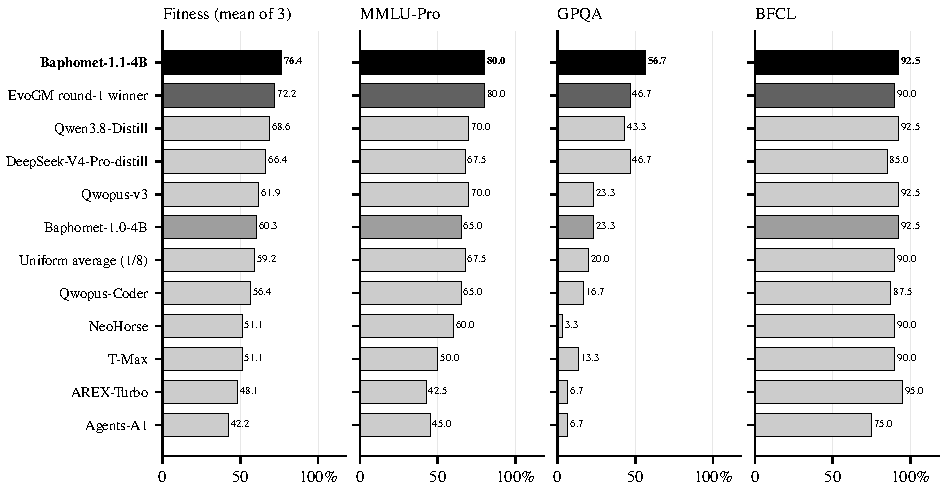
\includegraphics[width=\textwidth]{fig_fit110_acc_en.pdf}
\caption{Fitness and per-task accuracy on the 110-item fitness set for Baphomet-1.1-4B, the round-1 winner, the eight donors, Baphomet-1.0-4B and the uniform average. Baphomet-1.1 was selected on these items, so its score is optimistic.}
\label{fig:fit110}
\end{figure}

\begin{figure}[htbp]
\centering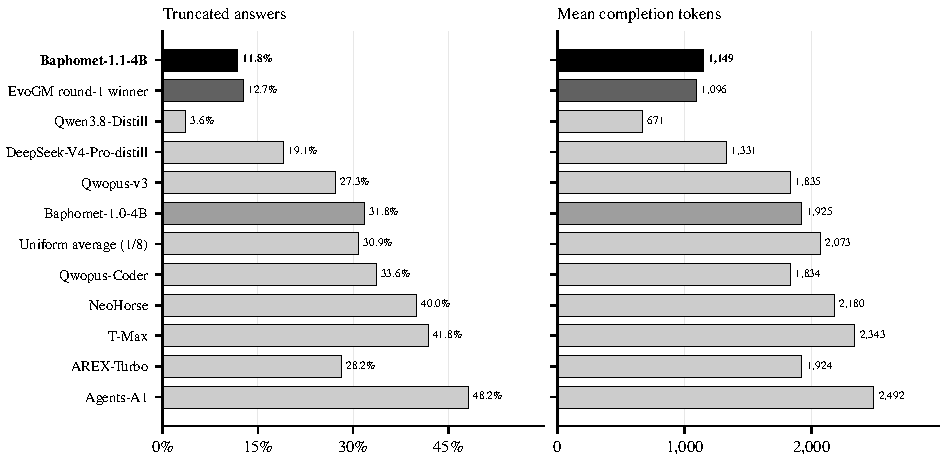
\includegraphics[width=\textwidth]{fig_fit110_eff_en.pdf}
\caption{Truncation rate and mean completion tokens on the 110-item fitness set (same models and order as Figure~\ref{fig:fit110}).}
\label{fig:fit110eff}
\end{figure}

\paragraph{Test set.} Table~\ref{tab:test} and Figure~\ref{fig:test} give the 180-item results for the four models run on the test (the donors and the uniform average were not). Baphomet-1.1 is numerically best overall (79.4\%, Wilson 95\% CI 73.0--84.7) ahead of Baphomet-1.0 (77.8\%, 71.2--83.2), the round-1 winner (77.2\%, 70.6--82.7) and Qwen3.5-4B (70.0\%, 62.9--76.2). The intervals overlap widely. In the paired test (Table~\ref{tab:mcnemar}) Baphomet-1.1 is \emph{not} significantly better than Baphomet-1.0 (10 items won, 7 lost, $p=0.63$) or than the round-1 winner (12 vs.\ 8, $p=0.50$), and is significantly better than the base model (20 vs.\ 3, $p<0.001$), mainly through GPQA (10 vs.\ 0, $p=0.002$) and MMLU-Pro (9 vs.\ 1, $p=0.021$). Per suite against Baphomet-1.0 it is ahead on MMLU-Pro (+3.8 points) and GPQA (+4.0) and behind on BFCL ($-4.0$, 0 vs.\ 2 discordant items), none significant.

\begin{table}[htbp]
\centering\small
\caption{180-item test (8{,}192-token cap). Acc.\ in \%; Trunc.\ $=$ share of truncated answers (\%); Tok.\ $=$ mean completion tokens. Donors were not run on this test.}
\label{tab:test}
\setlength{\tabcolsep}{4pt}
\begin{tabular}{llrrr}
\toprule
Suite ($n$) & Model & Acc. & Trunc. & Tok. \\
\midrule
MMLU-Pro (80) & \textbf{Baphomet-1.1-4B} & \textbf{81.3} & 5.0 & 1{,}492 \\
 & Round-1 winner & 75.0 & 5.0 & 1{,}200 \\
 & Baphomet-1.0-4B & 77.5 & 13.8 & 3{,}331 \\
 & Qwen3.5-4B & 71.3 & 17.5 & 4{,}385 \\
\midrule
GPQA (50) & \textbf{Baphomet-1.1-4B} & \textbf{62.0} & 28.0 & 4{,}007 \\
 & Round-1 winner & 62.0 & 16.0 & 3{,}270 \\
 & Baphomet-1.0-4B & 58.0 & 34.0 & 5{,}915 \\
 & Qwen3.5-4B & 42.0 & 54.0 & 7{,}094 \\
\midrule
BFCL (50) & \textbf{Baphomet-1.1-4B} & 94.0 & 0.0 & 207 \\
 & Round-1 winner & 96.0 & 0.0 & 202 \\
 & Baphomet-1.0-4B & \textbf{98.0} & 0.0 & 205 \\
 & Qwen3.5-4B & 96.0 & 0.0 & 229 \\
\midrule
All (180) & \textbf{Baphomet-1.1-4B} & \textbf{79.4} & 10.0 & 1{,}834 \\
 & Round-1 winner & 77.2 & 6.7 & 1{,}498 \\
 & Baphomet-1.0-4B & 77.8 & 15.6 & 3{,}180 \\
 & Qwen3.5-4B & 70.0 & 22.8 & 3{,}983 \\
\bottomrule
\end{tabular}
\end{table}

\begin{table}[htbp]
\centering\small
\caption{Paired comparison on the 180-item test: items only the first model got right -- items only the second got right, and the exact two-sided McNemar $p$.}
\label{tab:mcnemar}
\setlength{\tabcolsep}{4pt}
\begin{tabular}{lcccc}
\toprule
Comparison & All & MMLU-Pro & GPQA & BFCL \\
\midrule
Baphomet-1.1 vs.\ Baphomet-1.0 & 10--7 ($p$=.63) & 5--2 (.45) & 5--3 (.73) & 0--2 (.50) \\
Baphomet-1.1 vs.\ round-1 winner & 12--8 (.50) & 7--2 (.18) & 5--5 (1.0) & 0--1 (1.0) \\
Baphomet-1.1 vs.\ Qwen3.5-4B & 20--3 ($<$.001) & 9--1 (.021) & 10--0 (.002) & 1--2 (1.0) \\
Round-1 winner vs.\ Baphomet-1.0 & 8--9 (1.0) & 3--5 (.73) & 5--3 (.73) & 0--1 (1.0) \\
Baphomet-1.0 vs.\ Qwen3.5-4B & 17--3 (.003) & 7--2 (.18) & 9--1 (.021) & 1--0 (1.0) \\
\bottomrule
\end{tabular}
\end{table}

\begin{figure}[htbp]
\centering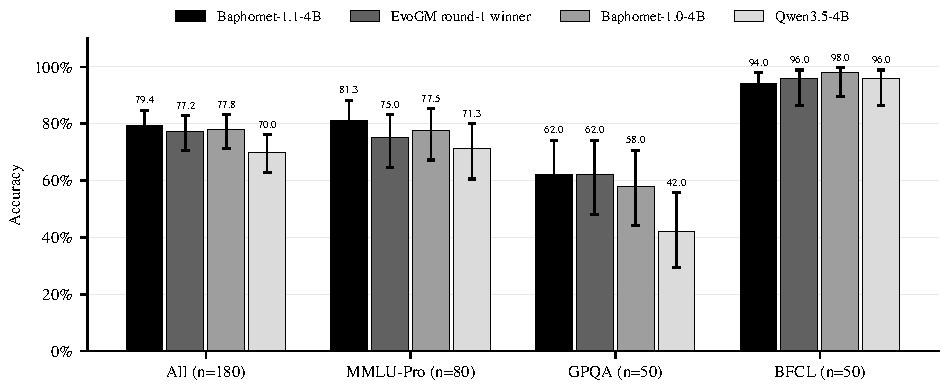
\includegraphics[width=\textwidth]{fig_test180_acc_en.pdf}
\caption{180-item test accuracy with Wilson 95\% confidence intervals (8{,}192-token cap). Only these four models were run on the test; the eight donors and the uniform average were not.}
\label{fig:test}
\end{figure}

\paragraph{Reasoning length.} Baphomet-1.1 generates 42\% fewer completion tokens than Baphomet-1.0 overall (1{,}834 vs.\ 3{,}180; 55\% fewer on MMLU-Pro, 32\% fewer on GPQA) and truncates less (10.0\% vs.\ 15.6\%). Compared with the round-1 winner, however, it is longer (1{,}834 vs.\ 1{,}498 tokens) and truncates more (10.0\% vs.\ 6.7\%), almost entirely on GPQA (28\% vs.\ 16\% truncated; Figure~\ref{fig:testeff}). Part of the accuracy gain over the round-1 winner was therefore bought with longer reasoning.

\begin{figure}[htbp]
\centering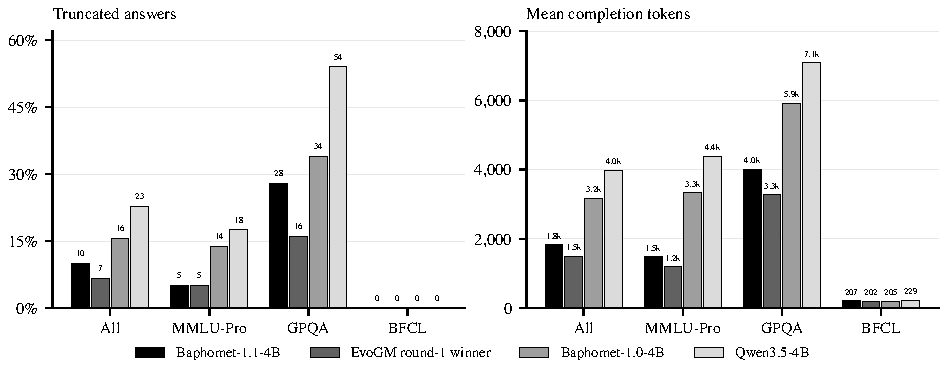
\includegraphics[width=\textwidth]{fig_test180_eff_en.pdf}
\caption{Truncation rate and mean completion tokens on the 180-item test.}
\label{fig:testeff}
\end{figure}

\section{Discussion}
\paragraph{What the extra rounds bought.} Two more rounds raised the best exact fitness from 0.722 to 0.764 and the test accuracy from 77.2\% to 79.4\%. Neither the test gain over the round-1 winner (12 vs.\ 8 discordant items) nor the one over Baphomet-1.0 (10 vs.\ 7) is significant. Baphomet-1.1 is the numerically best model we have measured, not a demonstrated improvement over Baphomet-1.0.

\paragraph{Winner's curse.} The winner is the maximum over many noisy measurements, so its measured value overstates its true quality. This happens twice here. First, the IRT estimate selected it for completion and overstated its exact fitness (0.782 vs.\ 0.764), as for the completed candidates on average ($+0.008$). Second, the exact 110-item fitness is itself a single sample at temperature 0.6 on a small item set, and the winner is the maximum of 52 exact values (40 round-1 candidates and 12 completions, the latter picked from 64 new candidates); part of its 0.042 lead over the round-1 winner on that set is likely selection noise. The 180-item test, which played no part in the selection, is the unbiased comparison, and there the lead shrinks to 2.2 points.

\paragraph{Efficiency.} Round 1 suggested that a capped generation fitness selects for short reasoning. Rounds 2--3 found a merge that is more accurate but somewhat longer than the round-1 winner (test: 1{,}834 vs.\ 1{,}498 tokens; GPQA truncation 28\% vs.\ 16\%), while still clearly shorter than Baphomet-1.0. At the 4{,}096-token fitness cap the two winners have similar lengths (1{,}149 vs.\ 1{,}096 tokens), so the difference appears mainly at the larger test cap.

\paragraph{IRT acceleration.} The 40-item estimator was accurate enough to steer the search (MAE 0.009, rank correlation 0.96 on completed candidates) at about 40\% of the tokens of a full evaluation. The completion rule kept the final choice on exact values, so the remaining IRT bias affects which candidates were completed, not the reported winner's fitness.

\paragraph{Fitness design matters.} Compared with the earlier log-likelihood search, which produced a merge that lost to Baphomet (2 vs.\ 17 discordant items on a 90-item subset) and broke tool calling, the generation-based fitness with a tool-use task produced merges that keep tool calling (BFCL 94--96\%) and match or exceed Baphomet-1.0. The runs differ in more than the fitness (merge method, donor count, search algorithm), so this comparison is suggestive only.

\section{Limitations}
One search with one seed; the 110-item fitness is one sample at temperature 0.6 and the winner was selected on it, so fitness-set comparisons with the donors are optimistic for Baphomet-1.1; candidates not completed (including the 3 stopped by racing) have only IRT estimates; the 180-item test is small (a 2--4-point difference is not significant); the donors and the uniform average were not run on the test; the fitness uses a shorter token cap than the test, and truncation explains part of every model's errors, so accuracies at a larger cap may differ; donor descriptions follow their model cards, which we did not verify.

\section{Conclusion}
An EvoGM-style search with a generation-based, token-capped fitness, continued for two rounds with an IRT-accelerated estimator under a further 6.53-GPU-hour run, produced Baphomet-1.1-4B. It is the best model on the fitness set (0.764 vs.\ 0.686 for the best donor and 0.603 for Baphomet-1.0, with selection bias in its favour) and numerically the best on the disjoint 180-item test (79.4\% vs.\ 77.8\% for Baphomet-1.0 and 70.0\% for Qwen3.5-4B), but not significantly better than Baphomet-1.0 ($p=0.63$). It uses 42\% fewer completion tokens than Baphomet-1.0. Next steps: a larger test set with several samples per item, accuracy--token budget curves (2k--16k), several search seeds, and test-set evaluation of the strongest donors.

\paragraph{Release.} Baphomet-1.1-4B is $\theta_0+\sum_i\lambda_{1.1,i}\tau_i$ with the coefficients above and base Qwen/Qwen3.5-4B. The released weights are reconstructed with the same fp8-quantized task vectors and the same merge code (\texttt{linmerge.py}) as the evaluated model, so they correspond to the weights tested here.

\paragraph{Compute.} Kaggle 2$\times$T4, vLLM 0.33.0. Round 1: 7.13 kernel hours (6.83\,h search, 0.3\,h test) plus 0.67\,h for a smoke test. Rounds 2--3: 6.53 kernel hours including setup, 64 subset evaluations, 12 completions and the 180-item test.

\small
\begin{thebibliography}{99}
\bibitem{evogm} T.~Jiang, X.~Yu, C.~Yi, Y.~Wu, Y.~Li, R.~Cheng, D.~Jiang, J.~Zhang. EvoGM: Learning to Merge LLMs via Evolutionary Generative Optimization. ICML 2026. arXiv:2605.29295.
\bibitem{evogmcode} EvoGM reference implementation. \url{https://github.com/JiangTao97/evogm}
\bibitem{qwen} Qwen/Qwen3.5-4B. \url{https://huggingface.co/Qwen/Qwen3.5-4B}
\bibitem{baph} CloudGoat/Baphomet-1.0-4B. \url{https://huggingface.co/CloudGoat/Baphomet-1.0-4B}
\bibitem{m1} InternScience/Agents-A1-4B. \url{https://huggingface.co/InternScience/Agents-A1-4B}
\bibitem{m2} Jackrong/DeepSeek-V4-Pro-Qwen3.5-4B. \url{https://huggingface.co/Jackrong/DeepSeek-V4-Pro-Qwen3.5-4B}
\bibitem{m3} empero-ai/Qwen3.8-4B-Distill. \url{https://huggingface.co/empero-ai/Qwen3.8-4B-Distill}
\bibitem{m4} Jackrong/Qwopus3.5-4B-Coder. \url{https://huggingface.co/Jackrong/Qwopus3.5-4B-Coder}
\bibitem{m5} Jackrong/Qwopus3.5-4B-v3. \url{https://huggingface.co/Jackrong/Qwopus3.5-4B-v3}
\bibitem{m6} BAAI/AREX-Turbo. \url{https://huggingface.co/BAAI/AREX-Turbo}
\bibitem{m7} TokenRhythm/NeoHorse-1-4B. \url{https://huggingface.co/TokenRhythm/NeoHorse-1-4B}
\bibitem{m8} allenai/tmax-4b. \url{https://huggingface.co/allenai/tmax-4b}
\end{thebibliography}
\end{document}
